\documentclass[conference]{IEEEtran}
\usepackage{bm}
\usepackage{bbm}
\usepackage{amsmath}
\usepackage{amsthm}
\usepackage{algorithm,algorithmic}
\usepackage{url}
\usepackage{authblk}
\usepackage{xcolor}
\usepackage{amssymb}
\usepackage{mathtools}
\usepackage{graphicx}
\DeclarePairedDelimiter\norm{\lVert}{\rVert}
\DeclareMathOperator{\Var}{Var}
\newtheorem{definition}{Definition}
\newtheorem{theorem}{Theorem}
\newtheorem{lemma}{Lemma}
\newtheorem{remark}{Remark}
\newtheorem{corollary}{Corollary}
\DeclareMathOperator{\SBMSI}{SBMSI}
\DeclareMathOperator{\SSBM}{SSBM}
\DeclareMathOperator{\SDP}{SDP}
\DeclareMathOperator{\Tr}{Tr}
\DeclareMathOperator{\E}{\mathbb{E}}
\DeclareMathOperator{\diag}{diag}
\DeclareMathOperator{\dist}{dist}
\DeclareMathOperator{\Bern}{Bern}
\DeclareMathOperator{\Binom}{Binom}
\DeclareMathOperator{\KL}{KL}
%\renewcommand{\baselinestretch}{0.98}
\newcommand{\A}{\frac{a \log(n)}{n}}
\newcommand{\B}{\frac{b \log(n)}{n}}
\title{Exact Recovery in the Balanced Stochastic Block Model with Side Information}
\author[1]{\textbf{Jin Sima}}
\author[2]{\textbf{Feng Zhao}}
\author[3]{\textbf{Shao-Lun Huang}}
\affil[1]{\normalsize{Department of Electrical Engineering, California Institute of Technology, Pasadena 91125, CA, USA}}
\affil[2]{\normalsize{Department of Electronic Engineering,
		Tsinghua University, 
		Beijing, China 100084}}
\affil[3]{\normalsize{DSIT Research Center,
		Tsinghua-Berkeley Shenzhen Institute,
		Shenzhen, China 518055}}
	\allowdisplaybreaks[4]
\begin{document}
	\maketitle
	\begin{abstract}
		The role that side information plays in improving the exact recovery threshold in the stochastic block model (SBM) has been studied in many aspects. This paper studies 
		exact recovery in $n$ node balanced binary symmetric SBM with side information, given in the form of $O(\log n)$ i.i.d. samples at each node. A sharp exact recovery threshold is obtained and turns out to coincide with an existing threshold result, where no balanced constraint is imposed. Our main contribution is an efficient semi-definite programming (SDP) algorithm that achieves the optimal exact recovery threshold. Compared to the existing works on SDP algorithm for SBM with constant number of samples as side information, the challenge in this paper is to deal with the number of samples increasing in $n$.	
		% The role that side information plays in improving the exact recovery threshold in the stochastic block model (SBM) has been studied in many aspects. This paper studies 
		% 	exact recovery in balanced binary symmetric stochastic block models with side information, given in the form of i.i.d. samples at each node.
		% 	The balanced constraint in the SBM allows us to derive a sharp exact recovery threshold that is analytical. We also present an efficient semi-definite programming (SDP) algorithm that achieves the optimal exact recovery threshold. Our SDP algorithm is a non-trivial generalization of the SDP algorithm for SBM without side information in the sense that our proof involves more detailed arguments. Moreover, the SDP algorithm also applies to the binary SBM where the label of each node has a uniform distribution.
	\end{abstract}
	\section{Introduction}
	The stochastic block model (SBM) \cite{holland1983stochastic}, also known as the planted partition model, is a statistical model that admits neat theoretical analysis and efficient algorithms while capturing some key features exhibited in large data networks, such as social, biological, and computer networks \cite{abbe2015exact}. 
	The SBM describes a graph of $n$ nodes, partitioned into multiple communities. Each edge in the graph exists independently with a probability determined by the communities the two nodes on the edge belong to. The goal is to recover  the community each node belongs to, based on one instance of the graph edges. While there are several levels of recovery defined and studied (see \cite{Abbe17} for a comprehensive survey), in this paper we focus on the exact recovery, which aims to recover all the communities. 
	
	For exact recovery in the SBM, a more interesting regime is when the edge connecting probabilities are in the order of $O(\frac{\log n}{n})$, in which circumstance there are phase transition phenomena for the exact recovery problem. 
	The tight threshold on the exact recovery in this setting was not established until the work of \cite{abbe2015exact,mossel2016}, where efficient and optimal algorithms based on semi-definite programming (SDP) were also provided. 
	The results in \cite{abbe2015exact,mossel2016} were generalized in \cite{abbe2015community} where the sharp threshold for multiple communities with asymmetric edge connecting probabilities is derived, and in \cite{Hajek16}, where optimal SDP algorithms for multiple communities and two communities with unequal community sizes are given.
	
	While the SBM focuses on graphical data only, it is natural to study the benefit of additional local data at the nodes, referred to as side information, to the exact recovery in the SBM. Such setting arises in applications where multi-modal data are observed. For example, in a social network, not only the interactions among people, but also the profile of each individual can be collected. It has been shown in many studies that side information such as node attributes or features \cite{zhang2016community,mossel2016local,saad2020recovering} can assist the community detection tasks. For exact recovery in the SBM with side information, the work of \cite{abbe17sideinfo} generalized \cite{abbe2015community} and derived a sharp threshold for exact recovery in the SBM with side information, given in the form of $\log n$ data samples at each node, drawn identically and independently  according to a probability distribution determined by the community the node belongs to. The community belongings are described by node labels, which are i.i.d. according to a probability distribution. 
	%The threshold in \cite{abbe17sideinfo} holds for general cases and is expressed in the form of an optimization problem, to which no closed form solution can be found. 
	The work of \cite{esmaeili2019exact,esmaeili2019community,saad2018community,esmaeili2019b,esmaeili2020a} considered variations where side information is given as partial revealed labels, noisy labels, or latent variables. SDP algorithms were presented to achieve the sharp threshold in \cite{esmaeili2019exact,esmaeili2019b,esmaeili2020a}.
	
	In this paper, we consider balanced binary symmetric SBM with side information in the form of $O(\log n)$ i.i.d. node samples, drawn according to a distribution determined by the community the node belongs to. The balanced property in this paper means that the two communities in the graph have equal sizes. The setting in this paper can be regarded as a special case of that in \cite{abbe17sideinfo}, with the difference that each node belongs to any one of the two communities with probability $\frac{1}{2}$ in \cite{Abbe17}, while a balanced constraint is imposed in this paper.  
	
	The contributions of this paper are as follows. 
	First, we derived a sharp threshold for the balanced SBM with side information. It turns out that the threshold in this paper coincides with that of \cite{abbe17sideinfo} for the special case of SBM with side information and without balanced constraint. 
	Our major contribution is an SDP based algorithm that achieves the threshold with high probability. Different from the SDP algorithms proposed in \cite{esmaeili2019exact,esmaeili2019b,esmaeili2020a}, where the side information consists of a constant number of samples, our SDP algorithm deals with cases where the number of samples is of order $O(\log n)$. Our SDP algorithm is a nontrivial generalization of the SDP algorithm in \cite{abbe2015exact} where a set of row and column constraints are imposed, to deal with the scaling of the number of samples. This poses challenges in analyzing the optimality of the proposed SDP algorithm, since the dual problem of the SDP relaxation becomes more complex.    
	%The latter cases pose challenges different from the former cases, and the algorithms in \cite{esmaeili2019exact,esmaeili2019b,esmaeili2020a} do not work in such cases.
	
	%Note that the admissibility of an SDP algorithm normally requires a balanced assumption \cite{abbe2015exact},
	%\cite{esmaeili2019community} or other assumptions that the community sizes are fixed \cite{Hajek16}.  To this end, we added more linear constraints to the SDP problem and the proof is more involved.
	
	The paper is organized as follows. 
	In Section \ref{s:model}, we introduce the model and present some definitions and lemmas needed throughout the paper. Section \ref{s:sharp} presents a sharp bound on exact recovery. In Section \ref{s:sdp}, we provide an SDP algorithm that achives the optimal threshold. Section \ref{section:experiment} provides simulation results for the SDP algorithm. Section \ref{s:conclusion} concludes the paper.
	
	
%	\newpage
%	In network analysis, community detection assigns discrete labels to each node of the graph based on the observation of graph edges.
%	In addition to edge information, extra node features are often available in real-world applications in the form of graph signal \cite{dong2020graph},
%	noisy labels \cite{mossel2016local}, or
%	feature vectors \cite{zhang2016community}. Combining the edge and node information, it is expected that better
%	accuracy can be achieved for community detection problems. Within this context, a central problem 
%	is to investigate the gain that extra information brings to the detection problem, compared to the case when only edge observation is available.
%	
%	% first paragraph: short intro to SBM and Ising model
%	To get theoretical insight into such a problem, it is often assumed that the graph is generated from a simple probabilistic model called Stochastic Block Model (SBM), in which the probability of edge existence is higher within the community than between different communities \cite{holland1983stochastic}. For the solely presence of SBM, the condition on exact recovery of community labels has been studied extensively and the phase transition property has been established \cite{abbe2015community, mossel2016}. For a special case of two community model,
%	the recovery condition is summarized as $\sqrt{a} - \sqrt{b} > \sqrt{2}$ when $a,b$ are parameters of SBM.
%	
%	With the presence of extra node information, the condition of exact recovery is improved
%	and generalized \cite{saad2018community, abbe17sideinfo}. However, previous study does not exactly quantify the contribution of side information and graph information. In contrast, this paper will fill the gap by considering a model of two-community SBM with extra node feature vectors. Our result generalizes
%	the exact recovery threshold to a condition $\gamma D_{1/2}(p_0 || p_1) + (\sqrt{a} - \sqrt{b})^2 > 2$
%	where the contribution of side information is coded in Renyi divergence.
%	
%	To achieve the exact recovery condition of SBM, semi-definite programming (SDP) is often utilized \cite{Hajek16}.
%	SDP relaxation can also be used for SBM with side information \cite{esmaeili2019exact}, and in this paper we show that a sub-optimal exact recovery condition
%	of our model is achievable by such method.
%	
%	This paper is organized as follows. In Section \ref{s:rw}, we review the previous works which are closely related with ours.
%	In Section \ref{s:model}, we introduce the model and present our main results.
%	Then the article concludes in Section \ref{s:conclusion} and
%	detailed proofs are provided in Section \ref{s:proof}.
%	
%	The following notations are used throughout this paper: 
%	the random undirected graph $G$ is written as $G(V,E)$ with vertex set $V$ and edge set $E$;
%	$V=\{1,\dots, n\} =: [n]$;
%	$\mathcal{X}$ is the alphabet
%	of the random variable $X$; $m$ is the number of samples generated at each node;
%	$\Bern(p)$ and $\Binom(n,p)$ represent Bernoulli
%	and Binomial distribution respectively; $f(n)=\omega(g(n))$(or $=o(g(n))$) means that $\lim_{n\to \infty} f(n) / g(n) = \infty $(or $=0$);
%	$\mathbbm{1}[A]$ is the indicator function for the event $A$; $W^n$ is the n-ary Cartesian power of the set $W$;
%	The Hamming distance of 
%	two $n$-dimensional vectors is written as $\dist(x,y):=\sum_{i=1}^n \mathbbm{1}[x_n\neq y_n]$ for $x,y\in \{\pm 1 \}^n$.
%	
%	\section{Related Works}\label{s:rw}
%	This work extends the model of two-community SBM considered in \cite{abbe2015community}.
%	Specifically, we assume the extra feature vectors of each node are independent samples, whose distribution depends on the label of the node.
%	This model has been studied in Section V-B of \cite{saad2018community}. However,
%	\cite{saad2018community} only got a weak conclusion, which says that the sample complexity of feature vectors
%	$m$ is required to be of order $O(\log n)$ for side information to take effects. In this paper, we obtain
%	a closed-form condition for exact recovery when $m=\gamma \log n$ for a positive constant $\gamma$.
%	
%	A general case of side information is studied
%	in \cite{abbe17sideinfo}. We emphasize that the model setting in Theorem 4 of \cite{abbe17sideinfo}
%	assumes that the node labels are independently generated  from $\Bern(\frac{1}{2})$ while the model
%	in this paper requires uniform distribution over the space $\sum_{i=1}^n Y_i = 0$ where $Y_i \in \{\pm 1 \}$ is the label of the $i$-th node.
%	Although these two settings are equivalent in
%	SBM model when $n$ is large, we observe that it differs when side information is available. Our assumption is easier to analyze due to some
%	symmetric property of node observations.
%	
%	Rényi divergence has been used in SBM in \cite{zhang2016} to characterize the weak recovery error bound. Both the dense and sparse graph are considered.
%	Within this paper, we use Rényi divergence to characterize
%	the contribution of side information to exact recovery error bound in these two cases.
	\section{Preliminaries}\label{s:model}
	A balanced binary symmetric SBM is defined by a random graph %$Z=\{Z_{i,j}\}_{1\le i<j\le n}$
	with $n$ nodes $\{1,\ldots,n\}$ and edges $Z=\{Z_{i,j}\}_{1\le i<j\le n}$, where $Z_{i,j}=1$ if nodes $i$ and $j$ are connected with an edge and $Z_{i,j}=0$ otherwise. 
	Each node $i\in\{1,\ldots,n\}$ is associated with a label $Y_i\in \{\pm 1\}$ such that the label $Y=(Y_1,\ldots,Y_n)$ is uniformly distributed over the space $\{Y:\sum^n_{i=1}Y_i=0\}$. The edges $\{Z_{i,j}\}_{1\le i<j\le n}$ are independently distributed Bernoulli random variables, where $Z_{i,j}=1$ with probability $p=a\frac{\log n}{n}$ for nodes $i,j$ with the same labels, i.e., $Y_i=Y_j$, and $Z_{i,j}=1$ with probability $q=b\frac{\log n}{n}$ if $Y_i\ne Y_j$. In this paper, it is assumed that $a>b$. 

	
	
	
	A balanced binary symmetric SBM with side information (SBMSI) is a generalization of the balanced SBM. In addition to the graph $Z$ and the labels $Y$, each node $i$ has $m=\gamma \log n$ data samples $X^i_{j}$, $i\in \{1,\ldots,n\}$, $j\in \{1,\ldots,m\}$, that are drawn identically and independently from distribution $P_0$ if $Y_i=1$ and from distribution $P_1$ if $Y_i=-1$. Note that the data samples $X^i_{j}$, $j\in \{1,\ldots,m\}$ are independent from $\{Z_{i,j}\}_{1\le i<j\le n}$ given the label $Y_i$ for any $i\in\{1,\ldots,n\}$. Hence, the joint probability distribution of $(\{Z_{i,j}\}_{1\le i<j\le n},\{X^i_{j}\}_{1\le i\le n,1\le j\le m})$ conditioned on $Y$ is
	\begin{align}\label{eq:lh}
		&P(x=\{x^i_{j}\}_{1\le i\le n,1\le j\le m},z=\{z_{i,j}\}_{1\le i<j\le n}| (y_1,\ldots,y_n)) \nonumber\\
		=& \prod_{1\le i,j\le n}P(z_{i,j}|y_i,y_j)\prod_{i=1}^n \prod_{j=1}^m P(x^i_j|y_i), 
	\end{align}
	where 
	\begin{equation*}
		P  (z_{i,j}=1|y_i,y_j) = \begin{cases}
			p & \text{if } y_i=y_j \\
			q & \text{if } y_i\ne y_j
		\end{cases},
	\end{equation*}
	and
	\begin{equation*}
		P(x^i_j|y_i) = \begin{cases}
			P_0(x^i_j) & y_i = 1 \\
			P_1(x^i_j) & y_i = -1
		\end{cases}
	\end{equation*}
	The conditional probability distribution $P(\{x^i_{j}\}_{1\le i\le n,1\le j\le m},\{z_{i,j}\}_{1\le i<j\le n}| y_1,\ldots,y_n)$ is determined by parameters $n$, $p$, $q$, $P_0$, and $P_1$. Hence, 
	the SBMSI is denoted as $\SBMSI(n,m,p,q,P_0,P_1)$.
	In $\SBMSI(n,m,p,q,P_0,P_1)$, the goal is to recover the unknown labels $Y$, given the graph $Z$ and the data samples $X$. In this paper, we consider exact recovery of $Y$, which is defined as follows.
	\begin{definition}[Exact Recovery for $\SBMSI(n,m,p,q,P_0,P_1)$]
		Let
		$(Z=\{Z_{i,j}\}_{1\le i<j\le n},Y,X=\{X^i_{j}\}_{1\le i\le n,1\le j\le m})$ be a graph $Z$, node labels $Y$, and node data samples $X$ be drawn from the distribution defined by $\SBMSI(n,m,p,q,P_0,P_1)$.
		Exact recovery is solvable if there exists an algorithm that takes $(Z,X)$ as inputs and outputs $\hat{Y}=\hat{Y}(Z,X)$ such that the error probability $P_e:=P(\hat{Y} \neq Y)$ goes to $0$ as $n$ increases.
	\end{definition}
	The following definition will be used throughout this paper and is a special case of the definition in \cite{abbe17sideinfo}. Define $I_+$ to be the Chernoff information
	between $\textrm{Pois}(\frac{a}{2},\frac{b}{2})\times \underbrace{P_0 \times \dots \times P_0}_{\gamma}$
	and $\textrm{Pois}(\frac{b}{2}, \frac{a}{2})\times \underbrace{P_1 \times \dots \times P_1}_{\gamma}$ where $\textrm{Pois}(\cdot,\cdot)$ represents the bivariant Poisson distribution. 
	
% 	The function $g(a,b,\epsilon)$ was defined in \cite{abbe2015exact} and characterizes the exponent of the probability that a sum of $\frac{n}{2}$ Bernouli random variables with probability $\frac{b\log n}{n}$ is larger than another sum of $\frac{n}{2}$ Bernouli random variables with by $\epsilon \log n$
	By computing the Karush–Kuhn–Tucker (KKT) conditions, we have the following lemma. %the proof of which can be found at the end of Section \ref{s:sdp}.  
	\begin{lemma}\label{lem:p0p12}
		For an $\SBMSI(n,m,p,q,P_0,P_1)$, let
		\begin{align}
			I_1=\min_{P_{\widetilde{X}_1}} \gamma D(P_{\widetilde{X}_1}|| P_0)+ \frac{1}{2} g(a,b, 2\epsilon),\text{ where}\nonumber\\
			\epsilon = \gamma \frac{D(P_{\widetilde{X}_1} || P_1) - D(P_{\widetilde{X}_1} || P_0) }{\log a /b}\label{eq:I1}\\
	   g(a,b,\epsilon) \triangleq a + b - \sqrt{\epsilon^2 + 4ab} + \epsilon \log \frac{\epsilon + \sqrt{\epsilon^2 + 4ab}}{2b}\label{equation:g}
		\end{align}
		and
		\begin{align}
			I_2=\min_{P_{\widetilde{X}_2}} \gamma D(P_{\widetilde{X}_2}|| P_1)+ \frac{1}{2} g(a,b, 2\epsilon),\text{ where}\nonumber\\
			\epsilon = \gamma \frac{D(p_{\widetilde{X}_2} || P_0) - D(P_{\widetilde{X}_2} || P_1) }{\log a /b}.\label{eq:I2}
		\end{align}
 		Then, we have that $I_1=I_2=I_+$. 
%If $p_0,p_1$
% 		satisfies
% 		\begin{equation}\label{eq:p0p1extra}
% 		    \sum_{x\in \mathcal{X}} \sqrt{p_0(x)p_1(x)}\log\frac{p_0(x)}{p_1(x)}=0
% 		\end{equation}
% 		$I_+$ has closed-form solution given by
% 		\begin{equation}\label{eq:IplusSpecial}
% 		    I_+=\frac{\gamma D_{1/2}(p_0||p_1) + (\sqrt{a}-\sqrt{b})^2}{2}
% 		\end{equation}
% 		where $D_{1/2}(p_0||p_1):=-2\log(\sum_{x\in\mathcal{X}} \sqrt{p_0(x)p_1(x)})$ is the Rényi divergence with order $\frac{1}{2}$
% 		between $p_0$ and $p_1$.
	\end{lemma}
	\begin{proof}
Using the results from Section 3 of \cite{abbe17sideinfo}, we can write $I_+$
explicitly as follows
\begin{align}\label{equation:I+}
    I_+ &=\frac{\lambda}{2} (a^{1-\lambda}b^{\lambda} -
    b^{1-\lambda}a^{\lambda})\log\frac{b}{a}+\frac{a+b}{2}\notag \\
    &-\frac{1}{2}(a^{1-\lambda}b^{\lambda} +
    b^{1-\lambda}a^{\lambda})+\gamma D_{\mathrm{KL}}(p_{\lambda}||p_0) 
	\end{align}
	where $\lambda$ is chosen to
	minimize
	\begin{equation}\label{eq:lambda}
     a^{1-\lambda}b^{\lambda} +
    b^{1-\lambda}a^{\lambda} + 2\gamma \log(\sum_{x\in \mathcal{X}}p^{1-\lambda}_0(x) p^{\lambda}_1(x))
\end{equation}
and $p_{\lambda}$ is defined as
\begin{equation}\label{eq:p12}
p_{\lambda}(x)= \frac{p_0^{1-\lambda}(x)p_1^{\lambda}(x)}{\sum_{x \in \mathcal{X}}p_0^{1-\lambda}(x) p_1^{\lambda} (x)}.
\end{equation}
We show that $I_1=I_+$ as an example.
The other part $I_2=I_+$ can be proved
similarly.
We use Lagrange multiplier to solve \eqref{eq:I1}.
Let
\begin{align*}
L(p_{\widetilde{X}_1},\epsilon, \lambda)
&=\gamma D(p_{\widetilde{X}_1}|| p_0)+ \frac{1}{2} g(a,b, 2\epsilon)\\
&- \lambda(\epsilon \log\frac{a}{b}-\gamma
D(p_{\widetilde{X}_1} || P_1) + \gamma D(p_{\widetilde{X}_1} || P_0))
\end{align*}
It is equivalent to minimize
$(1-\lambda)D(p_{\widetilde{X}_1} || P_0) +
\lambda D(p_{\widetilde{X}_1} || P_1) $, from
which we get $p_{\widetilde{X}_1}(x) = p_{\lambda}(x)$.
From $\frac{\partial L(p_{\widetilde{X}_1},\epsilon, \lambda)}{\partial \epsilon}=0$ and taking \eqref{eq:p12}
into \eqref{eq:I1}, we get
\begin{align*}
    \lambda \log \frac{a}{b}
    & = \log \frac{\epsilon + \sqrt{\epsilon^2+ab}}{b} \\
    \epsilon \log \frac{a}{b}
    & = \gamma\frac{\sum_{x \in \mathcal{X}}p_0^{1-\lambda}(x) p_1^{\lambda} (x)\log \frac{p_0(x)}{p_1(x)}}{\sum_{x \in \mathcal{X}}p_0^{1-\lambda}(x) p_1^{\lambda} (x)}
\end{align*}
After cancelling $\epsilon$
from the above two equations, we can get a single equation
for $\lambda$:
\begin{align*}
    &\frac{\log\frac{a}{b}}{2}
    (a^{\lambda} b^{1-\lambda}
    -a^{1-\lambda} b^{\lambda})
    + \gamma \frac{\sum_{x \in \mathcal{X}}p_0^{1-\lambda}(x) p_1^{\lambda} (x)\log \frac{p_1(x)}{p_0(x)}}{\sum_{x \in \mathcal{X}}p_0^{1-\lambda}(x) p_1^{\lambda} (x)}\\
    &=0
\end{align*}
which is the derivative of \eqref{eq:lambda}.
Then by simple computation we have
$I_+ = I_1$. 
%Furthermore,  if \eqref{eq:p0p1extra} is satisfied, $\lambda=\frac{1}{2}$
%is a solution of the above equation, and \eqref{eq:IplusSpecial} follows from
%\eqref{equation:I+} by letting $\lambda=\frac{1}{2}$.
\end{proof}
	\section{Sharp Threshold for Balanced SBMSI}\label{s:sharp}
	In this section we present a sharp closed form threshold for exact recovery in the balanced SBMSI. The threshold coincides with the result in \cite{abbe17sideinfo} for SBMSI without balanced constraints.  %We first provide the threshold, that comes from
	%the phase transition in the exact recovery in SBMSI with sparse graph structure. 
	\begin{theorem}\label{thm:Pe}
		For a balanced $\SBMSI(n,m,p=a\frac{\log n}{n},q=b\frac{\log n}{n},P_0,P_1)$, exact recovery is solvable if
		\begin{equation}\label{eq:positive_condition}
			I_+ > 1,
		\end{equation}
%			in which case, the error probability
%	\begin{equation*}
%		P_e \leq (1+o(1)) n^{-\frac{1}{2}\left(\gamma D_{1/2}(p_0||p_1) + (\sqrt{a} - \sqrt{b})^2-2\right)},
%	\end{equation*}
		and is not solvable if $I_+ < 1$, in which case, the error probability $P_e$ goes to $1$.
	\end{theorem}
	\begin{remark}
	From Lemma \ref{lem:p0p12}, 
	we can obtain $I_+ \geq \frac{1}{2}
	(\sqrt{a} - \sqrt{b})^2 +
	\frac{\gamma}{2} D_{\frac{1}{2}}(P_0||P_1)$.
	it can be seen that when $\gamma$ increases, in which case the number of samples becomes larger, a lower bound of $I_+$ increases. Hence, more samples facilitate the recovery of communities. 
	\end{remark}
% 	\begin{remark}
% 	Theorem \ref{thm:Pe} implies a separation of graph observation and side information, in the sense that the left part of \eqref{eq:positive_condition} is exactly the sum of the terms that appear in the exact recovery threshold in SBM  when there is graph observation only \cite{abbe2015exact} and when there is side information only, respectively. This separation is in contrast to the case in \cite{abbe17sideinfo}, where side information $X$ and graph observation $Z$ are coupled and a joint optimization in both $Z$ and $X$ with no closed form solution is needed. In Fig. \ref{fig:my_label} we show a comparison of our threshold and the one from \cite{abbe17sideinfo} when $P_0$ and $P_1$ are Bernoulli random variables with probability $ 0.05$ and $0.5$, respectively and $\gamma=5$.  It can be seen that there is a slight difference between the results in \cite{abbe17sideinfo} and in this paper.		We note that when such difference is small, our threshold can be used as an approximation to the threshold in \cite{abbe17sideinfo}, which is easily computable and provides insight to design the system. For example, when the parameters $a$ and $b$ are fixed in the graph, one can easily find the number of samples $m=\gamma\log n$ needed to achieve the exact recovery. 
% 	\end{remark}

	\subsection{Proof of Theorem \ref{thm:Pe}}
	%\begin{proof}[Proof of Theorem \ref{thm:Pe}]
% \color{red}
% 	The proof of Theorem \ref{thm:Pe} follows similar arguments to those in \cite{abbe2015exact}. We first show the first part of Theorem \ref{thm:Pe}, i.e., the achievability of exact recovery when \eqref{eq:positive_condition} holds. For any label $Y=(Y_1,\ldots,Y_n)$ satisfying $\sum^n_{i=1}Y_i=0$, let $A(Y)=\{i:Y_i=1\}$ and $B(Y)=\{i:Y_i=-1\}$ be the sets of nodes with labels $1$ and $-1$, respectively.  
% 	Let $Y^*=(y^*_1,\ldots,y^*_n)$ be the true labels of the nodes. We prove that with high probability, $Y^*$ is the output of an MAP (maximum a posteriori probability) estimator, which is equivalent to an ML (maximum likelihood) estimator since $Y$ is uniformly distributed over the space $\{Y:\sum^n_{i=1}Y_i=0\}$.
% 	Let $F_k$ be the event that there exists a labeling $Y'$ satisfying $|A(Y')\backslash A(Y)|=|B(Y')\backslash B(Y)|=k$. Then, by the union bound, it suffices to show that the probability $P(F_k)$ of the event $F_k$ is upper bounded by $o(\frac{1}{n})$ for anly $k\in\{1,\ldots,n\}$.
	
% 	Let $P_k$ be the maximum probability that 
% 	the likelihood $P(X,X| (Y^*_1,\ldots,Y^*_n)$ is smaller than the likelihood $P(X,Z| (Y'_1,\ldots,Y'_n))$, 
% 	over all labeling $Y'=(Y'_1,\ldots,Y'_n)$ satisfying $|A(Y')\backslash A(Y)|=|B(Y')\backslash B(Y)|=k$, where the likelihood $P(X,Z| (Y_1,\ldots,Y_n)$ is defined in \eqref{eq:lh}. Then by the union bound, we have that 
% 	\begin{equation}\label{eq:FAk}
% 		P(F_k) \leq \binom{n/2}{k}^2 P_k
% 	\end{equation}
% 	It remains to derive an upper bouond on $P_k$. 
% 	According to \eqref{eq:lh}, $P_k$ is the probability that
% 	\begin{align}\label{eq:ein}
% 		&\sum^m_{j=1}(\sum_{i\in A(Y^*)\backslash A(Y')} \log \frac{P_1(X^i_{j})}{P_0(X^i_{j})}
% 		+\sum_{i\in A(Y')\backslash A(Y^*)} \log \frac{P_0(X^i_{j})}{P_1(X^i_{j})})\nonumber\\
% 		\ge & \log \frac{p(1-q)}{q(1-p)} (\sum_{i\in A(Y^*)\backslash A(Y'),j\in A(Y^*)\cap A(Y')}z_{i,j}\nonumber\\
% 		&+\sum_{i\in A(Y')\backslash A(Y^*),j\in B(Y^*)\cap B(Y')}Z_{i,j}\nonumber\\
% 		&-\sum_{i\in A(Y^*)\backslash A(Y'),j\in B(Y^*)\cap B(Y')}Z_{i,j}\nonumber\\
% 		&-\sum_{i\in A(Y')\backslash A(Y^*),j\in A(Y^*)\cap A(Y')}Z_{i,j})
% 	\end{align}
% 	Note that the right hand side of \eqref{eq:lh} can be written as $\log \frac{p(1-q)}{q(1-p)}(Z_1-Z_2)$, where $Z_1\sim Binom(k(n-2k),\frac{a\log n}{n})$ and $Z_2\sim Binom(k(n-2k),\frac{b\log n}{n})$ 
% 	follow binomial distributions, where a binomial distribution $Binom(s,r)$ is the probability distribution of the sum of $s$ independent Bernouli random variables, each equals $1$ with probability $r$.
% 	The left hand side can be expressed as
% 	\begin{align*}
% 		\epsilon\triangleq&\log^{-1}( a /b)\cdot [\sum_{i\in A(Y^*)\backslash A(Y')}(D(P_{\widetilde{X}^i} || P_0) - D(p_{\widetilde{X}^i} || P_1)) \\
% 		&+ \sum_{i\in A(Y')\backslash A(Y^*)}(D(p_{\widetilde{X}^i} || P_1) - D(p_{\widetilde{X}^i} || P_0))],
% 	\end{align*}
% 	where $P_{\widetilde{X}^i}$ is the empirical distribution of samples $\{x^i_j\}^m_{j=1}$ at node $i$. 
	

% 		We start from \eqref{eq:ein}.
% 		Since $m=\gamma \log n$, $\sum_{i=1}^{km} \log \frac{p_1(x_{1i})}{p_0(x_{1i})} \sim
% 		-km D(p_0 || p_1)$, which is of order $O(\log n)$.
% 		Let $\epsilon$ be defined as follows:
		
		
% 		Then \eqref{eq:ein} is equivalent to
% 		\begin{equation}\label{eq:zeps}
% 			\sum_{i=1}^{k(n-2k)}(z'_{i} - z_{i}) \geq \epsilon \log n
% 		\end{equation}
% 		Using the type theory (11.1 of \cite{cover1999elements}), we can estimate the probability of the event $A_k$ given by \eqref{eq:zeps}.
% 		\begin{align}
% 			P(A_k) & =  \sum_{P^{(1)},P^{(2)}\in \mathcal{P}_{km}} Q_0^{km}(T(P^{(1)}))Q_1^{km}(T(P^{(2)}))\notag \\
% 			& \cdot P(\sum_{i=1}^{k(n-2k)} (z'_{i} - z_{i} \geq \epsilon(P^{(1)}, P^{(2)})  \log n ))\label{eq:decomp} 
% 		\end{align}
% 		Then using Theorem 11.1.4 of \cite{cover1999elements} and Lemma \ref{lem:zxt} 
% 		\begin{align*}
% 			&P(A_k)  \leq \sum_{P \in P_n} \exp(-km (D(p_{\widetilde{X}_1} || p_0) + D(p_{\widetilde{X}_2} || p_1))) \\
% 			& \cdot \exp(-\log n \frac{k(n-2k)}{n}\cdot (g(a, b, \frac{n}{k(n-2k)}\epsilon) + o(1))) \\
% 			&\leq |\mathcal{P}_{km}|^2 \exp(-k\log n \cdot (\theta^*_k + o(1))) 
% 		\end{align*}
% 		where
% 		\begin{align}
% 			\theta^*_k &= \min_{\widetilde{X}_1,\widetilde{X}_2} \gamma (D(p_{\widetilde{X}_1}|| p_0) + D(p_{\widetilde{X}_2} || p_1)) \notag \\
% 			&\quad + (1-\frac{2k}{n}) g(a,b, \frac{n}{k(n-2k)}\epsilon) \label{eq:theta_star}
% 		\end{align}
		
% 		By Lemma \ref{lem:p0p12}, we can get
% 		\begin{align}
% 			\theta^*_k &\geq (1-\frac{2k}{n})(\sqrt{a} - \sqrt{b})^2
% 			+ \frac{ \gamma}{2}\min (D(p_{\widetilde{X}_1}||p_0) + D(p_{\widetilde{X}_1}||p_1)) \notag \\
% 			&+ \frac{ \gamma}{2}\min (D(p_{\widetilde{X}_2}||p_0) + D(p_{\widetilde{X}_2}||p_1))\notag \\
% 			&=  (1-\frac{2k}{n})(\sqrt{a} - \sqrt{b})^2 - 2 \gamma\log(\sum_{x\in\mathcal{X}}\sqrt{p_0(x)p_1(x)}) 
% 			\label{eq:theta_star_lower_bound}
% 		\end{align}
% 		Next, we show that the lower bound is achievable.
% 		When the probability distribution of $\widetilde{X}_1, \widetilde{X}_2$ takes the form given by \eqref{eq:p012},
% 		$\epsilon = 0$, and $\theta^*_k$ in \eqref{eq:theta_star} is exactly the lower bound \eqref{eq:theta_star_lower_bound}.
% 		Since $\theta^*_k>0$,
% 		and $|\mathcal{P}_{km}|\leq (km+1)^{|\mathcal{X}|} $, we have $P(A_k) \leq n^{-k(\theta^*_k+o(1))}$.
		
% 		Using the union bound, we can control $P(F_k)$ by
% 		$$
% 		P(F_k) \leq \binom{n/2}{k}^2 P(A_k)
% 		$$
% 		When $k \geq \frac{n}{\sqrt{\log n}}$, using Lemma 8 of \cite{feng2021},
% 		$P(F_k)$ decreases exponentially. The error probability for $k < \frac{n}{\sqrt{\log n}}$
% 		is analyzed using \eqref{eq:FAk}.
% 		\begin{align*}
% 			&P_e \leq (1+o(1))\sum_{k=1}^{\frac{n}{\sqrt{\log n}}} P(F_k) \leq (1+o(1)) \cdot \\
% 			&\sum_{k=1}^{\frac{n}{\sqrt{\log n}}} \exp(k(-\mu \log n + \frac{2k}{n} \log n(\sqrt{a} - \sqrt{b})^2 - 2\log 2k + 2))
% 		\end{align*}
% 		where $\mu = (\sqrt{a} - \sqrt{b})^2-2 + \gamma D_{1/2}(p_0||p_1) > 0$.
% 		Using the inequality
% 		$$
% 		\frac{2k}{n}(\sqrt{a} - \sqrt{b})^2\log n -2\log2k+2\leq \frac{\mu}{2} \log n
% 		$$
% 		for $1\leq k \leq \frac{n}{\sqrt{\log n}}$, we can obtain
% 		\begin{align*}
% 			P_e &\leq(1+o(1)) \sum_{k=1}^{\frac{n}{\sqrt{\log n}}} \exp(k(-\mu \log n/2)) \\
% 			& =(1+o(1)) \frac{n^{-\mu / 2}}{1-n^{-\mu / 2}} = (1+o(1))n^{-\mu / 2}
% 		\end{align*}
% 		Therefore, \eqref{eq:PeMain} is established.
% \color{black}
%		\newpage
		The achievability part can be proved by our SDP algorithm, the details of which will be given in  Section \ref{s:sdp}.
		We show that exact recovery is not possible if $I_+ < 1$. %Most parts of the arguments follow a similar manner to those in \cite{abbe2015exact}.
		
		Let $S_1$ and $S_2$ be the set of nodes with labels $1$ and $-1$, respectively. For a node $i$ and a node set $S\subset\{1,\ldots,n\}$,
		let $E(i,S)$ be the number of edges between $i$ and nodes in $S$.
		By similar arguments to the ones in \cite{abbe2015exact}, it can be shown that with high probability, there exists a subset
		 $H_1\subset S_1$ of size $\frac{n}{\log^3 n}$ and a node $i_1\in H_1$, such that  
		\begin{align}
			\sum_{j=1}^{m} \log \frac{P_1(x^{i_1}_{j})}{P_0(x^{i_1}_{j})}
			\ge &\log \frac{p(1-q)}{q(1-p)}\Big(\frac{\log n}{\log\log n}+1\nonumber\\
			&+E(i_1, S_1 \backslash H_1) - E(i_1, S_2) \Big) \label{eq:G1},
		\end{align}	
	if $I_1<1$, where $I_1$ is defined in \eqref{eq:I1}. Similarly, if $I_2<1$, where $I_2$ is defined in \eqref{eq:I2}, there exists a subset
		$H_2\subset S_2$ of size $\frac{n}{\log^3 n}$ and a node $i_2\in H_2$, such that  
		\begin{align}
			\sum_{j=1}^{m} \log \frac{P_0(x^{i_2}_{j})}{P_1(x^{i_2}_{j})}
			\ge &\log \frac{p(1-q)}{q(1-p)}\Big(\frac{\log n}{\log\log n}+1\nonumber\\
			&+E(i_2, S_2 \backslash H_2) - E(i_2, S_1) \Big) \label{eq:G2},
		\end{align}	
	with high probability. Summing up \eqref{eq:G1} and \eqref{eq:G2}, we obtain	
		\begin{align}
			&\sum_{j=1}^{m} \log \frac{P_1(x^{i_1}_{j})}{P_0(x^{i_1}_{j})}
			+\sum_{j=1}^{m} \log \frac{P_0(x^{i_2}_{j})}{P_1(x^{i_2}_{j})}\nonumber\\    
			\ge &\log \frac{p(1-q)}{q(1-p)}\Big(2\frac{\log n}{\log\log n}+2+E(i_1, S_1 \backslash H_1) \nonumber\\
			&+ E(i_2, S_2 \backslash H_2)- E(i_1, S_2 ) - E(i_2, S_1 )\Big) \label{eq:G1ij}.
		\end{align}	
		Note that if \eqref{eq:G1ij} holds, then
		\begin{align}
			&\sum_{j=1}^{m} \log \frac{P_1(x^{i_1}_{j})}{P_0(x^{i_1}_{j})}
			+\sum_{j=1}^{m} \log \frac{P_0(x^{i_2}_{j})}{P_1(x^{i_2}_{j})}\nonumber\\
			\ge &\log \frac{p(1-q)}{q(1-p)}(E(i_1, S_1 \backslash \{i_1\}) + E(i_2, S_2 \backslash \{i_2\})\nonumber\\
			&- E(i_1, S_2 \backslash \{i_2\}) - E(i_2, S_1 \backslash \{i_1\})) \label{eq:F1ij}.
		\end{align}
		Hence, with high probability, \eqref{eq:F1ij} holds if $I_1<1$ and $I_2<1$. According to Lemma \ref{lem:p0p12}, this occurs when $I_+<1$. According to \eqref{eq:lh} and the fact that $Y$ is uniformly distributed, Eq. \eqref{eq:F1ij} is equivalent to the fact that the likelihood $P(X,Z|(Y_1,\ldots,Y_n))$ (defined in \eqref{eq:lh}) with $Y_{i_1}=-1,Y_{i_2}=1$ is larger than the likelihood $P(X,Z|(Y_1,\ldots,Y_n))$ with $Y_{i_1}=1,Y_{i_2}=-1$, which results in  recovery failure. Therefore, we conclude that a recovery failure occurs with high probability, if $I_+<1$.  

		
% 		By the definition and property of $H_1$ and $H_2$ mentioned above, the probability of \eqref{eq:F1ij} is lower bounded by the probability of

% 		Let $G_1(i_1)$ and $G_2(i_2)$ be the events that
% 		\begin{align*}
% 			\sum_{j=1}^{m} \log \frac{P_1(x^{i_1}_{j})}{P_0(x^{i_1}_{j})}
% 			\ge &\log \frac{p(1-q)}{q(1-p)}\Big(\frac{\log n}{\log\log n}\\
% 			&+E(i_1, S_1 \backslash H_1) 
% 			- E(i_1, S_2 \backslash \{i_2\}\Big)		    
% 		\end{align*}
		
% 		that \eqref{eq:G1ij} holds for any $i_1\in H_1$ and $i_2\in H_2$.
% 		In the next, we show that
% 		the probability of $G(i_1,i_2)$ is lower bounded by $\frac{1}{n^{-2+\mu}}$ for some positive constant $\mu$. Then we have that 
% 		\begin{align}
% 			& P(\cap_{i_1\in S_1, i_2\in S_2} F^c(i_1,i_2)) \le P(\cap_{i_1\in H_1, i_2\in H_2} G^c(i_1,i_2)) \nonumber\\
% 			& = (1 - P(G(i_1,i_2)))^{|H_1|\cdot|H_2|}\nonumber\\
% 			& \leq (1-n^{-2+u})^{n^2/\log^6 n} \nonumber\\
% 			& \leq \exp(-n^{\mu+ o(1)}) \to 0, \label{eq:boundg}
% 		\end{align}
% 		where $F^c(i_1,i_2)$ and $G^c(i_1,i_2)$ are the events that $F(i_1,i_2)$ and $G(i_1,i_2)$ do not occur,respectively. Eq. \eqref{eq:boundg} implies that with high probability $F(i_1,i_2)$ occurs for some $i_1\in S_1$ and $i_2\in S_2$, and hence the failure occurs.
		
% 		Note that the right hand side of \eqref{eq:G1ij} is upper bounded by $\log \frac{p(1-q)}{q(1-p)}(Z_1-Z_2+o(\log n))$, where $Z_1\sim \Binom(n-2,\frac{a\log n}{n})$ and $Z_2\sim \Binom(n-2,\frac{b\log n}{n})$ 
% 		follow binomial distributions. A binomial distribution $\Binom(s,r)$ is the probability distribution of the sum of $s$ independent Bernoulli random variables, each equals $1$ with probability $r$.
% 		The left hand side can be expressed as
% 		\begin{align*}
% 			\epsilon\triangleq&m\log^{-1}( a /b)\cdot [(D(P_{\widetilde{X}^{i_1}} || P_0) - D(P_{\widetilde{X}^{i_1}} || P_1)) \\
% 			&+(D(P_{\widetilde{X}^{i_2}} || P_1) - D(P_{\widetilde{X}^{i_2}} || P_0))],
% 		\end{align*}
% 		where $P_{\widetilde{X}^i}$ is the empirical distribution of samples $\{x^i_j\}^m_{j=1}$ at node $i$. Let $P_{\widetilde{X}^{i_1}}$ and $P_{\widetilde{X}^{i_2}}$ follow the distribution specified in \eqref{eq:p012}. Then we have that $\epsilon =0$. Using Sanov's theorem and Lemma 4 from \cite{abbe2015exact}, we have that
% 		\begin{align*}
% 			&P(G(i_1,i_2))\\
% 			\geq &\frac{1}{(m+1)^{2|\mathcal{X}|}} \exp(-m(D(p_{\widetilde{X}_1} || p_0) + D(p_{\widetilde{X}_2} || p_1)) \\
% 			&\cdot\exp(- (\sqrt{a} - \sqrt{b})^2\log n+o(\log n) ) \\
% 			& = \exp(-\log n (\gamma D_{1/2}(P_0||P_1) + (\sqrt{a} - \sqrt{b})^2+ o(1))),
% 		\end{align*}
% 		where $\mathcal{X}$ is the alphabet of distributions $P_0$ and $P_1$.
% 		Since $\gamma D_{1/2}(P_0||P_1) + (\sqrt{a} - \sqrt{b})^2<2$, we have that $P(G(i_1,i_2))\ge n^{-2+\mu}$ for some positive constant $\mu$.
%	\end{proof}
	

	
	\section{SDP Relaxation}\label{s:sdp}
	In this section, we propose a semi-definite programming based relaxation to find the maximum likelihood estimate of the labels $Y$. Note that
	the ML estimate of the labels $Y$ is NP-hard while
	SDP formulation can be implemented efficiently using
	interior point method
	or alternating direction method of multipliers \cite{boyd2011distributed}.
	Our SDP algorithm finds the true label $Y^*$ with probability approaching $1$, if
	$I_+ > 1$.
	The SDP problem can be solved using various efficient iterative schemes.
	
	Let $S_1(Y)$ and $S_2(Y)$ be the sets of nodes with label $1$ and $-1$, respectively, given $Y$.
	According to \eqref{eq:lh}, the log likelihood of $Y$ is given by
	\begin{align}\label{eq:loglh}
		&\sum^m_{j=1}[\sum_{i\in S_1(Y)} \log P_0(X^i_{j})+\sum_{i\in S_2(Y)} \log P_1(X^i_{j})]\nonumber\\
		&+\sum_{i,j\in S_1(Y),i<j}[z_{i,j}\log p+(1-z_{i,j})\log (1-p)]\nonumber\\
		&+\sum_{i,j\in S_2(Y),i<j}[z_{i,j}\log p+(1-z_{i,j})\log (1-p)]
		\nonumber\\
		&+\sum_{i\in S_1(Y),j\in S_2(Y)}[z_{i,j}\log q+(1-z_{i,j})\log (1-q)].
	\end{align}
	It can be verified that maximizing \eqref{eq:loglh} over $Y\in\{\pm 1\}^n$ is equivalent to solving the following optimization problem
	\begin{align}
		\max_{v}\, & h^T v + \frac{1}{4}v^T B v \notag \\
		s.t.\, & \mathbbm{1}_n^T v = 0 \text{ and } v_i \in \{\pm 1 \} \label{eq:matrix_mle}
	\end{align}
	where $h$ is an n-dimensional vector with entry $h_i = \frac{1}{\log \frac{p(1-q)}{q(1-p)}}\sum_{j=1}^m \log \frac{P_0(x^i_{j})}{P_1(x^i_{j})}$ for $i\in\{1,\ldots,n\}$ and the $n\times n $ matrix $B$ is defined as
	\begin{equation}
		B_{ij} = \begin{cases}
			1, & \text{if $i$ is connected to $j$}, \\
			-1,& \text{otherwise.}
		\end{cases}
	\end{equation}  
	for $i,j\in\{1,\ldots,n\}$.
	%However, we find that
	%the maximal solution is unchanged when $\kappa$ takes other values as long as $\kappa > b\frac{\log %n}{n}$.
	
	Let $v^*$ be the optimal solution to \eqref{eq:matrix_mle} and $V^*=(1,v^*)(1,v^*)^T$, where $(1,v^*)$ is a $(n+1)$-dimensional  vector obtained by concatenating $1$ and $v^*$.
	Then, the optimal value of \eqref{eq:matrix_mle} equals $\frac{1}{2}Tr(\widetilde{B}V^*)$, where
	\begin{equation}\label{eq:B_lambda_def}
		\widetilde{B} = \begin{pmatrix} 0 & h^T  \\ h  & \frac{1}{2}B \end{pmatrix}.
	\end{equation}
	We wish to show that $V^*$ is the unique optimal solution to the following problem.
	\begin{align}
		\max_V\, Tr(\tilde{B}V)  &\notag\\
		s.t.\, V_{ii} &= 1, \notag\\
		V &\succeq 0, \notag\\
\sum_{j=2}^{n+1} (V_{ij} + V_{ji})& = 0,~\forall i\in\{1,\ldots,n+1\}. \label{eq:sdp}
	\end{align}
	Note that here we use $n+1$ constraints in the last line of \eqref{eq:sdp} to describe the balanced property of the labels. This is important in deriving the optimality and uniqueness of $V$, which will be proved in the following theorem. The theorem shows that our SDP relaxation achieves exact recovery with high probability, as long as the recovery condition is met.
	%When $m=0$ and $\kappa=1$,
	%the SDP is exactly the one Abbe considered in \cite{abbe2015exact}.
	%When $m=0$ and $\kappa=\frac{a-b}{\log a/b}\frac{\log n}{n}$, the SDP is
	%the same as the one in Theorem 3 of \cite{Hajek16}.
	% The theoretical guarantee for the relaxation form in \eqref{eq:sdp} is summarized
	% in the following theorem:
	\begin{theorem}\label{thm:sdp}
		If $I_+ > 1$, then with high probability, the optimal solution
		$V^*$ to \eqref{eq:sdp} is unique and given by $(1,y^*)(1,y^*)^T$, where $y^*$ is the true labeling of the nodes.
	\end{theorem}
	\begin{proof}[Proof of Theorem \ref{thm:sdp}]
	Consider the dual problem of \eqref{eq:sdp}
	\begin{align}
		\min_{a_1, \dots, a_{n+1}}\, &\sum_{i=1}^{n+1} a_i \nonumber\\\label{eq:dual}
		s.t. &\, \diag\{a_1, \dots, a_{n+1}\} + \Xi - \widetilde{B} \succeq 0, 
	\end{align}
	where the $(n+1)\times (n+1)$ symmetric matrix $\Xi$ is defined as 
	\begin{equation}
		\Xi_{ij} = \begin{cases}
			\lambda_1, & i=1\text{ or }j=1 \text{, and }i\ne j\\
			\lambda_i + \lambda_j, & i, j\in\{2,\ldots,n+1\}
		\end{cases},
	\end{equation}
	Let $g=y^*=(1,\ldots,1,-1,\ldots,-1)$ be the true labels of the nodes, i.e., the first and second half of the nodes are labeled by $1$ and $-1$, respectively. As similarly mentioned in \cite{abbe2015exact},
	the optimality and uniqueness of the solution $(1,g)(1,g)^T$ to \eqref{eq:sdp} is guaranteed by the following conditions: 
	\begin{enumerate}
		\item[(a)] $(1,g)(1,g)^T$ is a feasible solution to the primal problem \eqref{eq:sdp}.
		\item[(b)] There exists a feasible solution $(a_1,\ldots,a_{n+1},$ $\lambda_1,\ldots,\lambda_{n+1})$ to \eqref{eq:dual}, such that $\sum_{i=1}^{n+1} a_i=Tr((1,g)(1,g)^T\widetilde{B})$.
		\item[(c)] $(\diag\{a_1, \dots, a_{n+1}\} + \Xi - \widetilde{B})(1,g)=0$.
		\item[(d)] The second smallest eigenvalue of $\diag\{a_1, \dots, a_{n+1}\} + \Xi - \widetilde{B}$ is greater than $0$. 
	\end{enumerate}
	Condition (a) holds by definition. It suffices to choose $(a_1,\ldots,a_{n+1},\lambda_1,\ldots,\lambda_{n+1})$ that satisfies conditions (b), (c) and (d).
	Let $\mu=\frac{1}{n}\mathbbm{1}_n^T h$ and $\lambda = -\mu/n$. Specify $(a_1,\ldots,a_{n+1},$ $\lambda_1,\ldots,\lambda_{n+1})$ as follows
	$$\lambda_1=\mu+\lambda, \text{ and }\lambda_{i+1}=g_i\lambda + \lambda,~i\in\{1,\ldots,n\}$$
	Then, from condition (c) we have that
	\begin{align}
		a_1 &= h^T g \nonumber\\
		a_{i+1} & = (h_i -\lambda)g_i  + \frac{1}{2}\diag\{Bgg^T\}_i, i = 1, \dots, n
	\end{align}
	It can be verified that $\sum_{i=1}^{n+1} a_i = 2h^Tg +\frac{1}{2} g^T B g$, and hence condition (b) holds.
	Hence it suffices to prove that
	\begin{align}
		&\diag(\{a_1, \dots, a_{n+1}\}) + \Xi - \widetilde{B} \nonumber\\
		=& \begin{pmatrix} h^T g & -h^T +(\mu + \lambda)\mathbbm{1}_n^T \\
			-h+(\mu + \lambda )\mathbbm{1}_n & \Xi_n \end{pmatrix}
		\succeq 0, 
	\end{align}
	where
	\begin{align}\label{eq:Xi_n}
		\Xi_n =&\diag(hg^T + Agg^T -\lambda \mathbbm{1}_ng^T)  \nonumber\\
		&+ (\frac{1}{2} +2\lambda) J_n  - A + 2\lambda \Xi',
	\end{align}
	$\mathbbm{1}_n$ is the all 1's vector, $J_n$ is the all 1's matrix, and $I_n$ is the identity matrix. The matrix $A=(B+J_n-I_n)/2$ is the adjacency matrix of the graph.
	The matrix $\Xi'$ is given by $\Xi'_{ij}=g_i + g_j$.
	
	In the following we show that $\Xi_n$ is positive definite. Then according to condition (c) and the
	Cauchy's Interlacing Theorem \cite{hwang}, condition (d) holds.
	Then, the proof is done.
	
	We show that $x^T \Xi_n x>0$ for any vector $x \in \mathbb{R}^n$ satisfying $\norm{x}=1$. Decompose $x$ as $x=\frac{\beta}{\sqrt{n}} g
	+ \sqrt{1-\beta^2} g^{\perp}$, where $g^Tg^{\perp}=0, \beta \in [0,1]$, and $\norm{g^{\perp}}=1$. Then, we have that 
	\begin{align}
		x^T \Xi_n x = \frac{\beta^2}{n} g^T \Xi_n g  &
		+		\frac{\beta}{\sqrt{n}}\sqrt{1-\beta^2} g^T \Xi_n g^{\perp}
		\nonumber\\\label{eq:xax}
		&+
		(1-\beta^2)(g^{\perp})^T \Xi_n g^{\perp}. 
	\end{align}
	In the next we derive lower bounds to the three terms in the right hand side of \eqref{eq:xax}.
	For the first term, we have that
	\begin{align*}
		g^T \Xi_n g = g^T(h -\lambda \mathbbm{1}_n)   = g^T h
	\end{align*}
	Since $\mathbb{E}[g^T h]$ is a positive number of order $O(n\log n)$ ,
	by Sanov's theorem or Chernoff bound, the probability 
	$P(g^T h < 0)$ decreases exponentially in $n$. Hence, with high probability, the first term $g^T \Xi_n g$ is positive.
	
	For the second term, let $\tilde{h}=\Xi_n g
	=(n-1)\lambda\mathbbm{1}_n+h$, then
	$g^T \Xi_n g^{\perp} = \tilde{h}^T g^{\perp} \geq -\norm{\tilde{h}-\frac{1}{n}(\tilde{h}^Tg)g}$, where the  norm $\norm{\tilde{h}-\frac{1}{n}(\tilde{h}^Tg)g}$ satisfies
	\begin{align*}
		\norm{\tilde{h}-\frac{1}{n}(\tilde{h}^Tg)g}^2
		=\norm{\tilde{h}}^2 - \frac{1}{n}(\tilde{h}^Tg)^2.
	\end{align*}
	Let $\hat{g}_1 = \frac{1}{2}(g + \mathbbm{1}_n)$ and $\hat{g}_2 = \frac{1}{2}(-g +\mathbbm{1}_n)$.
	Using the fact that $\tilde{h}^T\mathbbm{1}_n=\mu$, we have 
	\begin{align*} 
		&\frac{\norm{\tilde{h}}^2}{n} - (\frac{1}{n}\tilde{h}^Tg)^2\\
		&=\frac{\norm{\tilde{h}}^2}{n} - 2\frac{(\tilde{h}^T \hat{g}_1)^2}{n^2} - 2\frac{(\tilde{h}^T \hat{g}_2)^2}{n^2} + \frac{(\tilde{h}^T\mathbbm{1}_n)^2}{n^2} \\
		&=2\frac{ \sum_{i<j,i,j\in S_1} (\tilde{h}_i - \tilde{h}_j)^2 + \sum_{i<j,i,j\in S_2} (\tilde{h}_i - \tilde{h}_j)^2 }{n^2}+ \frac{\mu^2}{n^2}\\
		& = I_1 + I_2 + \frac{\mu^2}{n^2}.
	\end{align*}
	where $I_j=\frac{\sum_{i\in S_j} h_i^2}{n} - 2\frac{(h^T \hat{g}_j)^2}{n^2}$ for $j\in\{1,2\}$,  and $S_1$ and $S_2$ denotes the sets of nodes with label $1$ and
	$-1$, respectively. Denote $\mathbb{E}[h_i]=m D_j, \Var[h_i]=m \bar{D}_j, \mathbb{E}[h_i^2]=\Var[h_i]+\mathbb{E}^2[h_i]=m \bar{D}_j+m^2 D^2_j, \Var[h_i^2] \leq m^4 \bar{C}_j$ for $i\in S_j$ and $j\in\{1,2\}$. Then
	$D_j, C_j,j\in\{1,2\}$ are constants.
	Using Chebyshev's inequality, we have that
	\begin{align*}
		P(\Big| \frac{\sum_{i\in S_j} h_i^2}{n} - \frac{1}{2}(m \bar{D}_j + m^2D_j^2) \Big| \geq \log n) & \leq \frac{m^4 \bar{C}_j}{2n\log^2 n} \\
		P(\Big| \frac{h^T \hat{g}_j}{n} - \frac{m}{2}D_j\Big| \geq \log^{-1} n) & \leq \frac{\bar{D}_j m \log^{2} n}{2n}
	\end{align*}
	for $j\in\{1,2\}$. Hence, with probability $1-n^{-1-o(1)}$, 
	\begin{align*}
		I_j \leq& \frac{1}{2}m\bar{D}_j + \frac{1}{2}m^2 D_j^2 + \log n - 2(\frac{1}{2}m D_j - \log^{-1} n)^2 \\
		=& O(\log n)
	\end{align*}
	for $j\in\{1,2\}$.
	Therefore, we have that
	$$
	\frac{1}{\sqrt{n}} g^T \Xi_n g^{\perp} \geq -\sqrt{\frac{\norm{\tilde{h}}^2}{n} - (\frac{1}{n}\tilde{h}^Tg)^2} = O(\sqrt{\log n})
	$$
 
 
	
	
	
	
	
	
	For the last term $(g^{\perp})^T \Xi_n g^{\perp}$, by \eqref{eq:Xi_n} and the fact that $(g^{\perp})^Tg=0$, we have that
	\begin{align*}
		&(g^{\perp})^T \Xi_n g^{\perp} \\
		=& (g^{\perp})^T \diag( -\lambda \mathbbm{1}_ng^T+hg^T + Agg^T) g^{\perp} + p \\
		&+ \frac{1}{2}(1-p-q+2\lambda)(g^{\perp})^TJ_n g^{\perp}
		-(g^{\perp})^T(A-\mathbb{E}[A])g^{\perp},
	\end{align*}
	where we use the fact that $\mathbb{E}[A] = \frac{p-q}{2}gg^T + \frac{p+q}{2}J_n - pI_n$. Note that $p,q,$ and $\lambda$ are $o(1)$ terms and that $(g^{\perp})^TJ_n g^{\perp}\ge 0$. 
	By Theorem 5.2 of \cite{lei2015consistency},
	with probability $1-n^{-r}$, $\lambda_{\max}(A-\mathbb{E}[A]) \leq c\sqrt{\log n}$ for some positive constant $r$ and $c$. Hence, we have that
	\begin{align}\label{eq:lastterm}
		(g^{\perp})^T \Xi_n g^{\perp} \geq \min_i\{(-\lambda + h_i) g_i+  g_i (Ag)_i \} - c \sqrt{\log n}
	\end{align}
	% The error probability is then bounded by
	% \begin{align*}
	% P(\Xi_{ii} \leq c\sqrt{\log n}, \forall 1\leq i \leq n)
	% \end{align*}
	We now show that with high probability,
	\begin{align}\label{eq:nodei}
		(-\lambda + h_i) g_i+  g_i (Ag)_i  - c \sqrt{\log n}\ge 0
	\end{align}
	for $i\in\{1,\ldots,n\}$. For $g_i=1$,
	the term $g_i(Ag)_i$ can be written as 
	$Z_1-Z_2$, where $Z_1\sim \Binom(\frac{n}{2}-1,\frac{a\log n}{n})$
	and $Z_2\sim \Binom(\frac{n}{2},\frac{b\log n}{n})$ 
	follow binomial distributions. The term $h_i=m \frac{D(P_{\widetilde{X}_i} || P_1) - D(P_{\widetilde{X}_i} || P_0) }{\log a /b}$, where $P_{\widetilde{X}_i}$ is the empirical distribution of samples $\{X^i_j\}^m_{j=1}$ at node $i$. Then, we have the following lemma, which is a slight generalization of Lemma 8 in \cite{abbe2015exact} and can be proved using Chernoff bound.
	\begin{lemma}\label{lem:zxt}
		Suppose $m > n, Z \sim \Binom(m, \frac{b\log n}{n}), X\sim \Binom(m, \frac{a\log n}{n})$.
		For $ t \geq \frac{m}{n}(b - a)$, we have
		\begin{align}\label{eq:estimation}
			&P(Z - X \geq t \log n) \nonumber\\
			\leq &\exp(-\frac{m}{n}\log n \cdot ( g(a, b, \frac{n}{m}t) + O(\frac{\log n}{n})))
		\end{align}
		where $g(a,b,\epsilon)$ is defined in \eqref{equation:g}.
	\end{lemma}
	According to Lemma \ref{lem:zxt} and Sanov's theorem, if $g_i=1$, the probability that \eqref{eq:nodei} does not hold is upper bounded by
	$n^{-I_1 + o(1)}$ for any $i$, where $I_1$ is defined in \eqref{eq:I1}. By the union bound, the probability that there exists an $i$ that violates \eqref{eq:nodei} is at most $n^{-I_1+1 + o(1)}$, which fades to zero as $I_1=I_+>1$. 
	Similarly, the probability that an $i$ satisfying $g_i=-1$ violates \eqref{eq:nodei} decays if $I_2=I_+>1$. Therefore, with high probability, $(g^{\perp})^T \Xi_n g^{\perp}\ge0$ when $I_+>1$, and Theorem \ref{thm:sdp} holds. 
\end{proof}
	% , and Theorem \ref{thm:sdp} gives a quantification of its theoretical
	% performance. For observations from binary symmetric channel, the result is
	% \begin{corollary}
	% 	Suppose $X_{ij}$ is the output of $Y_i$ from a binary symmetric channel with crossover probability
	% 	$p^*$. $P(\hat{Y}_{\SDP} \neq  Y) = o(1)$ as long as
	% 	\begin{equation}
	% 	-2\log(2\sqrt{p^*(1-p^*)}) + (\sqrt{a} - \sqrt{b})^2>2
	% 	\end{equation}
	% \end{corollary}
 	\section{Simulation Results}\label{section:experiment}
 	Fig. \ref{fig:my_label} shows the empirical probability of successful recovery of the SDP algorithm 
 	for the SBM with side information. We fix $n=300$ and the number of trials to be 20. The number of samples is chosen as $m=10$ for $\Bern(0.2)$ versus $\Bern(0.8)$. Then
 	at each trial and for fixed $a$ and $b$, we check how many times each method succeeds. Dividing
 	by the number of trials, we obtain the empirical probability of success with respect to
 	the exact recovery metric. The blue curve corresponds to the threshold $\sqrt{a}-\sqrt{b}=\sqrt{2}$ while the red curve  corresponds to the threshold $I_+ = 1$. It can be seen
 	from the figure that the recovery threshold
 	for SBM with side information matches the red line $I_+ = 1$.
 	\begin{figure}
 	    \centering
 	    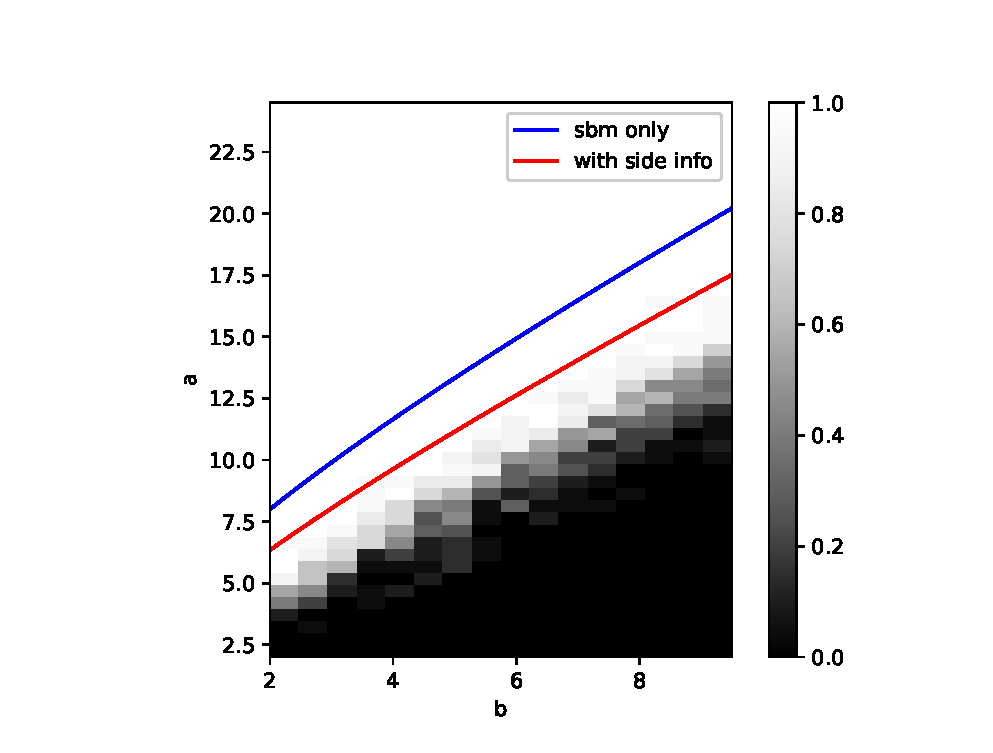
\includegraphics[width=0.5\textwidth]{new_results.eps}
 	    \caption{Comparison of different thresholds with empirical recovery result by SDP}
 	    \label{fig:my_label}
 	\end{figure}
	\section{Conclusion}\label{s:conclusion}In this paper, we obtained a sharp close-form exact recovery condition for a balanced two-community symmetric SBM with side information. %This condition
	%shows that the detection error can be %characterized by a separation of Rényi divergence and the parameters of SBM. To control the recovery error within a given level,
	Our result provides insight on the number of node samples to achieve exact recovery. We also proposed a semidefinite programming based algorithm that achieves the threshold with high probability. It will be interesting to see if the SDP algorithm in this paper can be extended to more general cases.
	\bibliographystyle{IEEEtran}
	\bibliography{exportlist}
\end{document}